
\tikzstyle{process} = [rectangle, minimum width=3cm, minimum height=1cm, text centered, draw=black]
\tikzstyle{arrow} = [thick,->,>=stealth]

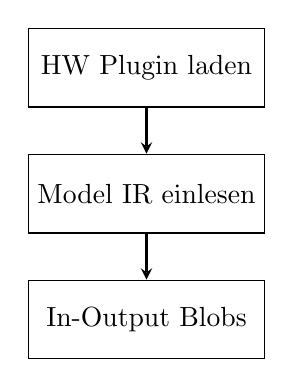
\begin{tikzpicture}[node distance=1.6cm]
    \node (start) [process] {HW Plugin laden};
    \node (mitte) [process, below of=start] {Model IR einlesen};
    \node (end) [process, below of=mitte] {In-Output Blobs};
    \draw [arrow] (mitte) -- (end);
    \draw [arrow] (start) -- (mitte);
\end{tikzpicture}
